%\documentclass[handout]{beamer}
\documentclass{beamer}

\usetheme{boxes} %see http://www.deic.uab.es/~iblanes/beamer_gallery/ for lots of examples
\usecolortheme{rose}
\useinnertheme{circles}
\useoutertheme{split}
\setbeamertemplate{blocks}[rounded][shadow=true]

\setbeamertemplate{navigation symbols}{}%remove navigation symbols

%next set colors - not needed
\setbeamercolor{title}{fg=black!70!black}
\setbeamercolor{frametitle}{fg=red!70!black}
\setbeamercolor{framesubtitle}{fg=green!30!black}
\setbeamercolor{author}{fg=red!70!black}
\setbeamercolor{institute}{fg=green!30!black}
\setbeamercolor{date}{fg=blue!50!black}

\usepackage[slovene]{babel}
\usepackage[OT2,T1]{fontenc}
\usepackage[utf8]{inputenc}
\usepackage{amsmath,amssymb,amsfonts,amsthm}
\usepackage{unicode-math}
\usepackage{colortbl}
%\usepackage[all]{xy}
%\usepackage{graphicx}
\usepackage{bm}

\newtheorem{izrek}[theorem]{Izrek}
\newtheorem{trditev}[theorem]{Trditev}
\newtheorem{posledica}[theorem]{Posledica}
\newtheorem{vprasanje}[theorem]{Vpra\v anje}
\newtheorem{domneva}[theorem]{Domneva}
\newtheorem{definicija}{Definicija}
\newtheorem{zgled}{Zgled}
\newtheorem{lema}[theorem]{Lema}


\beamertemplatetransparentcovereddynamic

\title{DPH krivulje}
\author{Simon Besednjak}
\institute{Fakulteta za matematiko in fiziko}
\date{32.13.2022}


% Matematični ukazi
\newcommand{\iu}{\mathrm{i}\mkern1mu}
\newcommand{\R}{\mathbb R}
\newcommand{\N}{\mathbb N}
\newcommand{\Z}{\mathbb Z}
\renewcommand{\C}{\mathbb C}
\newcommand{\Q}{\mathbb Q}
\newcommand{\quat}{\mathbb H}
\newcommand{\tangenta}{\frac{\mathbf{r}'}{\lVert \mathbf{r}'\rVert}}
\newcommand{\normala}{\frac{\mathbf{r}'\times\mathbf{r}''}{\lVert \mathbf{r}'\times\mathbf{r}'' \rVert}\times \mathbf{t}}
\newcommand{\binormala}{\frac{\mathbf{r}'\times\mathbf{r}''}{\lVert \mathbf{r}'\times\mathbf{r}'' \rVert}}
\newcommand{\fleksija}{\frac{\lVert \mathbf{r}'\times\mathbf{r}'' \rVert}{\sigma^3}}
\newcommand{\torzija}{\frac{(\mathbf{r}'\times\mathbf{r}'')\cdot\mathbf{r}'''}{\lVert \mathbf{r}'\times\mathbf{r}'' \rVert^2}}
\newcommand{\tV}{\mathbf{t}}
\newcommand{\aV}{\mathbf{a}}
\newcommand{\bV}{\mathbf{b}}
\newcommand{\cV}{\mathbf{c}}
\newcommand{\dV}{\mathbf{d}}
\newcommand{\eV}{\mathbf{e}}
\newcommand{\fV}{\mathbf{f}}
\newcommand{\hV}{\mathbf{h}}
\newcommand{\nV}{\mathbf{n}}
\newcommand{\pV}{\mathbf{p}}
\newcommand{\qV}{\mathbf{q}}
\newcommand{\rV}{\mathbf{r}}
\newcommand{\iV}{\mathbf{i}}
\newcommand{\jV}{\mathbf{j}}
\newcommand{\kV}{\mathbf{k}}
\newcommand{\uV}{\mathbf{u}}
\newcommand{\vV}{\mathbf{v}}
\newcommand{\wV}{\mathbf{w}}
\newcommand{\zV}{\mathbf{z}}
\newcommand{\ndr}{\lVert \mathbf{r}'\rVert} % norma prvega odvoda
\newcommand{\ndrtddr}{\lVert \mathbf{r}'\times \mathbf{r}'' \rVert} % norma vektorskega produkta prvega in drugega odvoda
\newcommand{\AQ}{\mathcal{A}}
\newcommand{\BQ}{\mathcal{B}}
\newcommand{\CQ}{\mathcal{C}}
\newcommand{\DQ}{\mathcal{D}}
\newcommand{\QQ}{\mathcal{Q}}
\newcommand{\VQ}{\mathcal{V}}
\newcommand{\UQ}{\mathcal{U}}
\newcommand{\balpha}{\symbf{\alpha}}
\newcommand{\bbeta}{\symbf{\beta}}
\newcommand{\bgamma}{\symbf{\gamma}}
\newcommand{\bdelta}{\symbf{\delta}}
\newcommand{\brho}{\symbf{\rho}}
\newcommand{\btau}{\symbf{\tau}}
\newcommand{\btalpha}{\tilde{\symbf{\alpha}}}
\newcommand{\btbeta}{\tilde{\symbf{\beta}}}
\newcommand{\bell}{\symbf{\ell}}
\newcommand{\dFrac}[2][t]{\frac{\mathrm{d}#2}{\mathrm{d}#1}} %odvod, default spremenljivka je t

% \DeclareMathOperator{\tr}{tr}  % morda potrebuješ operator za sled ali kaj drugega?
\DeclareMathOperator{\st}{st}
\DeclareMathOperator{\hopf}{H}
\DeclareMathOperator{\ReC}{Re}
\DeclareMathOperator{\ImC}{Im}
\DeclareMathOperator{\nhopf}{\hat{H}}


\begin{document}
%%%%%

\frame{\titlepage}
%%%%%%%%%%%%%%%%%%%%%%%%%%%%%%%%%%%%%%%%%%%%
\frame{
	\frametitle{Parametrično podane prostorske krivulje}
	\pause
	\begin{equation*}
		\rV:I \to \R^3, I \subseteq \R, \quad \rV(t)=(x(t),y(t),z(t)), \quad t \in I,
	\end{equation*}
	\pause
	\begin{equation*}
		\rV':I \to \R^3, \quad \rV'(t)=(x'(t),y'(t),z'(t)), \quad t \in I,
	\end{equation*}
	\pause
	$$\sigma(t)=\lVert \rV'(t)\rVert=\sqrt{x'^2(t)+y'^2(t)+z'^2(t)},$$
	\pause
	$$\tV=\frac{\rV'}{\lVert\rV'\rVert},\quad\pV=\frac{\rV'\times \rV''}{\lVert \rV'\times \rV'' \rVert} \times\frac{\rV'}{\lVert\rV'\rVert},\quad\bV=\frac{\rV'\times \rV''}{\lVert \rV'\times \rV'' \rVert},$$
	\pause
	$$\kappa=\frac{\lVert \rV' \times \rV'' \rVert}{\sigma^3}=\frac{\lVert \rV' \times \rV'' \rVert}{\lVert \rV' \rVert^3},\quad\tau=\frac{\big(\rV'\times\rV''\big)\cdot\rV'''}{\lVert \rV'\times \rV'' \rVert^2}.$$
}
%%%%%%%%%%%%%%%%%%%%%%%%%%%%%%%%%%%%%%%%%%%%
\frame{
	\frametitle{Krivulje s pitagorejskim hodografom}
	\begin{definicija}
		Prostorska polinomska krivulja $\rV:I \to \R^3,$ $\rV(t)=(x(t),y(t),z(t)),$ kjer je $I$ zaprt interval v $\R^3,$ ima \emph{pitagorejski hodograf}, če obstaja tak realen polinom $\sigma,$ da velja
		\begin{equation*}
			%\label{pitagorejski}
			x'^2(t)+y'^2(t)+z'^2(t)=\sigma^2(t),\quad t\in I.
		\end{equation*}
	\end{definicija}
	Takim krivuljam pravimo tudi \emph{PH krivulje}.
}
%%%%%%%%%%%%%%%%%%%%%%%%%%%%%%%%%%%%%%%%%%%%
\frame{
	\frametitle{Krivulje s pitagorejskim hodografom}
	\begin{izrek}
		Prostorska krivulja $\rV$ je PH krivulja natanko takrat, ko je njen hodograf oblike
		\begin{align*}
			x'(t)&=\big(u^2(t)+v^2(t)-p^2(t)-q^2(t)\big)w(t),\\
			y'(t)&=2\big(u(t)q(t)+v(t)p(t)\big)w(t),\\
			z'(t)&=2\big(v(t)q(t)-u(t)p(t)\big)w(t),
		\end{align*}
		za realne polinome $u,v,p,q$ in $w.$ \pause Parametrična hitrost se poenostavi v
		\begin{align*}
			\sigma(t)=\lVert\rV'(t)\rVert&=x'^2(t)+y'^2(t)+z'^2(t)\\
			&=\big(u^2(t)+v^2(t)+p^2(t)+q^2(t)\big)w(t).
		\end{align*}
		Pri tem polinom $w$ predstavlja skupni faktor komponent hodografa.
	\end{izrek}
}
%%%%%%%%%%%%%%%%%%%%%%%%%%%%%%%%%%%%%%%%%%%%
\frame{
	\frametitle{Krivulje s pitagorejskim hodografom - lastnosti}
	%\begin{itemize}
		%\item
		 Ločna dolžina regularne PH krivulje je v polinomski odvisnosti od parametra $t$:
			$$s(t)=\int_a^t\lVert\rV'(\xi)\rVert d\xi=\int_a^t\sigma(\xi)d\xi.$$
			\pause
			%\item 
			Enotska tangenta $\tV$ je racionalna funkcija parametra $t.$
			\pause
			%\item 
			$$\lVert\rV'\times\rV''\rVert^2=\sigma^2\rho,$$ kjer je $$\rho=4\big((up'-u'p+vq'-v'q)^2+(uq'-u'q+vp'-v'p)^2\big).$$
			\pause
			%\item 
			Torzijska ukrivljenost $\tau$ je racionalna funkcija parametra $t.$ V splošnem izrazi za $\kappa,\pV$ in $\bV$ niso racionalne funkcije parametra $t.$
	%\end{itemize}
}
%%%%%%%%%%%%%%%%%%%%%%%%%%%%%%%%%%%%%%%%%%%%
\frame{
	\frametitle{Kvaternionska oblika PH krivulj}
	\pause
	$$\AQ(t)=u(t)+v(t)\iV+p(t)\jV+q(t)\kV.$$
	\pause
	$$\AQ^*(t)=u(t)-v(t)\iV-p(t)\jV-q(t)\kV.$$
	\pause
	\begin{align*}
		\AQ(t)\iV\AQ^*(t)&=\big(u^2(t)+v^2(t)-p^2(t)-q^2(t)\big)\iV\\
		&+2\big(u(t)q(t)+v(t)p(t)\big)\jV\\
		&+2\big(v(t)q(t)-u(t)p(t)\big)\kV.
	\end{align*}
	\pause
	Velja: $\rV'=\AQ\iV\AQ^*.$
	\pause
	\begin{align*}
	\lVert \rV'(t) \rVert=\sigma(t)=\lVert \AQ(t) \rVert^2&=\AQ(t) \AQ^*(t)\\
	&=u^2(t)+v^2(t)+p^2(t)+q^2(t).
	\end{align*}
}
%%%%%%%%%%%%%%%%%%%%%%%%%%%%%%%%%%%%%%%%%%%%
\frame{
	\frametitle{Hopfova oblika PH krivulj}
	\pause
	\begin{definicija}	
		\emph{Hopfova preslikava} $H$ je preslikava, ki slika iz $\C \times \C \to \R^3$ in je za $\balpha, \bbeta \in \C$ določena z naslednjim predpisom:
		\begin{equation*}
			\hopf(\balpha, \bbeta)=(|\balpha|^2-|\bbeta|^2,2\ReC(\balpha \bar{\bbeta}),2\ImC(\balpha \bar{\bbeta})).
		\end{equation*}
	\end{definicija}
	\pause
	$$\balpha(t)=u(t)+\iu v(t),\quad\bbeta(t)=q(t)+\iu p(t).$$
	\pause
	Velja: 
	\begin{align*}
		\rV'(t)&=\hopf(\balpha(t),\bbeta(t)),\\
		\pause
		\lVert\rV'(t)\rVert&=|\balpha(t)|^2+|\bbeta(t)|^2.
	\end{align*}
}
%%%%%%%%%%%%%%%%%%%%%%%%%%%%%%%%%%%%%%%%%%%%
\frame{
	\frametitle{DPH krivulje}
	\pause
	\begin{definicija}	
		\label{dvojnaPH}
		Za prostorsko polinomsko krivuljo $\rV$ pravimo, da je \emph{DPH krivulja}, če sta tako $\lVert \rV' \rVert$ kot $\lVert \rV' \times \rV'' \rVert$ polinomski funkciji parametra $t,$ torej če sta izpolnjena pogoja
		\begin{equation*}
			\lVert \rV' \rVert^2=x'^2+y'^2+z'^2=\sigma^2,
		\end{equation*}
		\begin{equation*}
			\label{DPH_pogoj}
			\lVert \rV' \times \rV'' \rVert^2=(y'z''-y''z')^2+(z'x''-z''x')^2+(x'y''-x''y')^2=(\sigma \omega)^2
		\end{equation*}
		za neka polinoma $\sigma$ in $\omega.$ %Pogoju \eqref{DPH_pogoj} pravimo \emph{DPH pogoj}.
	\end{definicija}
	\pause
	Frenetovo ogrodje $(\tV,\pV,\bV)$ in fleksijska ukrivljenost $\kappa$ ter torzijska ukrivljenost $\tau$ so racionalno parametrizirane v parametru $t.$
}
%%%%%%%%%%%%%%%%%%%%%%%%%%%%%%%%%%%%%%%%%%%%
\frame{
	\frametitle{Vijačnice}
	\pause
	\begin{definicija}
		\label{definicija_vijacnica}
		Krivulja $\rV$ je vijačnica, če oklepa njena enotska tangenta $\tV$ konstanten kot $\psi$ (kjer je $0<\psi \leq \frac{\pi}{2}$) z nekim fiksnim enotskim vektorjem $\aV.$ Vektor $\aV$ predstavlja os vrtenja vijačnice.
	\end{definicija}
	\pause
	Ker sta vektorja $\aV$ in $\tV$ enotska, potem velja
	\begin{equation*}
		\label{pogoj_vijacnica}
		\aV \cdot \tV=\cos \psi.
	\end{equation*}
	\pause
	\begin{izrek}[Lancret]
		\label{lancret}
		Krivulja z neničelno fleksijsko ukrivljenostjo je vijačnica natanko takrat, ko je za vse njene točke razmerje med torzijsko in fleksijsko ukrivljenostjo konstantno.
	\end{izrek}
}
%%%%%%%%%%%%%%%%%%%%%%%%%%%%%%%%%%%%%%%%%%%%
\frame{
	\frametitle{DPH krivulje in vijačnice}
	\pause
	\begin{trditev}
		\label{trditev_vijacnica_DPH}
		Če je polinomska krivulja vijačnica, potem je tudi DPH krivulja.
\end{trditev}
	\pause
	\begin{izrek}
		\label{DPH_helix_3ali5}
		Polinomska krivulja stopnje tri ali pet je vijačnica natanko tedaj, ko je DPH krivulja.
	\end{izrek}
	\pause
	Za DPH krivulje razmerje med fleksijsko in torzijsko ukrivljenostjo enako
	\begin{equation*}
		\label{DPH_razmerje_ukrv_omega_mesani}
		\frac{\kappa}{\tau}=\frac{\omega^3}{(\rV'\times\rV'')\cdot\rV'''}%=\tan\psi.
	\end{equation*}
}
%%%%%%%%%%%%%%%%%%%%%%%%%%%%%%%%%%%%%%%%%%%%
\frame{
	\frametitle{DPH krivulje in vijačnice}
	\pause
	\begin{itemize}
		\item Vsaka PH krivulja stopnje 3 je hkrati vijačnica in hkrati DPH krivulja.
		\pause
		\item DPH krivulje stopnje 5 (ki so hkrati tudi vijačnice) predstavljajo pravo podmnožico množice PH krivulj stopnje 5.
		\pause
		\item Za stopnje 7 ali več predstavlja množica DPH krivulj pravo podmnožico množice PH krivulj. Obstajajo tako vijačne kot nevijačne DPH krivulje.
	\end{itemize}
}
%%%%%%%%%%%%%%%%%%%%%%%%%%%%%%%%%%%%%%%%%%%%
\frame{
	\frametitle{Polinom proporcionalnosti}
	\pause
	\begin{definicija}
		Polinomu $\balpha(t)\bbeta'(t)-\balpha'(t)\bbeta(t)$, ki ga sestavimo iz polinomov $\balpha(t)=u(t)+\iu v(t)$ ter $\bbeta(t)=q(t)+\iu p(t)$ za neke realne polinome $u(t),v(t),q(t)$ ter $p(t),$ pravimo tudi \emph{polinom proporcionalnosti} polinomov $\balpha(t)$ in $\bbeta(t)$.
	\end{definicija}
	\pause
	$$\rho=4|\balpha\bbeta'-\balpha'\bbeta|^2.$$
	\pause
	DPH pogoj:
	$$\balpha\bbeta'-\balpha'\bbeta=h\wV^2,$$
	kjer je $h$ realen polinom, $\wV$ pa kompleksen polinom.
}
%%%%%%%%%%%%%%%%%%%%%%%%%%%%%%%%%%%%%%%%%%%%
\frame{
	\frametitle{Normalizirana Hopfova preslikava}
	\pause
	\begin{equation*}
		\label{tangenta_hopf}
		\tV=\frac{\rV'}{\lVert\rV'\rVert}=\frac{\hopf(\balpha,\bbeta)}{|\balpha|^2+|\bbeta|^2}=\frac{(|\balpha|^2-|\bbeta|^2,2\ReC(\balpha\bar{\bbeta}),2\ImC(\balpha\bar{\bbeta}))}{|\balpha|^2+|\bbeta|^2}.
	\end{equation*}
	\pause
	\begin{definicija}
		\label{norm_hopf_def}
		\emph{Normalizirana Hopfova preslikava} je preslikava, ki slika iz $\C\times\C\to\R^3$ in ima naslednji predpis za $\balpha,\bbeta\in\C$:
		\begin{equation*}
			\label{norm_hopf}
			\nhopf(\balpha,\bbeta)=\frac{(|\balpha|^2-|\bbeta|^2,2\ReC(\balpha\bar{\bbeta}),2\ImC(\balpha\bar{\bbeta}))}{|\balpha|^2+|\bbeta|^2}.
		\end{equation*}
	\end{definicija}
	\pause
	Velja:
	\pause $$(|\balpha|^2+|\bbeta|^2)^2=(|\balpha|^2-|\bbeta|^2)^2+(2\ReC(\balpha\bar{\bbeta}))^2+(2\ImC(\balpha\bar{\bbeta}))^2.$$
	\pause $$\nhopf(\balpha/\bbeta,1)=\nhopf(\balpha,\bbeta)\quad\text{za}\quad\bbeta\neq0.$$
}
%%%%%%%%%%%%%%%%%%%%%%%%%%%%%%%%%%%%%%%%%%%%
\frame{
	\frametitle{Vijačnice in Hopfova preslikava}
	\pause
	Preslikava $\zV\to\nhopf(\zV,1)$ je inverz stereografske projekcije.
	\pause
	\begin{trditev}
		\label{vijacnica_slika_tangente}
		Slika enotske tangente %splošne
		vijačnice na (enotski) sferi tvori krožnico.
	\end{trditev}
	\pause
	\begin{itemize}
		\item Izberemo taka kompleksna polinoma $\balpha(t)$ in $\bbeta(t),$ katerih razmerje $\zV(t)=\balpha(t)/\bbeta(t)$ nam poda racionalno parametrizacijo premice oziroma krožnice v $\C.$
		\pause
		\item Slika premice oziroma krožnice z normalizirano Hopfovo preslikavo je torej krožnica na $S^2,$ torej je po trditvi pripadajoča krivulja res vijačna.
	\end{itemize}
}
%%%%%%%%%%%%%%%%%%%%%%%%%%%%%%%%%%%%%%%%%%%%
\frame{
	\frametitle{Konstrukcija vijačnic}
	\pause
	\begin{equation*}
		\label{transformacija}
		\zV(t)=\frac{\aV_0(1-t)+\aV_1t}{\bV_0(1-t)+\bV_1t},
	\end{equation*}
	kjer so $\aV_0,$ $\aV_1,$ $\bV_0$ in $\bV_1$ kompleksna števila, za katera velja $\aV_0\bV_1-\aV_1\bV_0\neq 0.$\pause
	
	Dva različna načina za konstrukcijo vijačnic:
	\begin{itemize}
		\pause
		\item Pomnožimo števec in imenovalec zgornjega izraza s kompleksnim polinomom, da dobimo $\zV(t)=\balpha(t)/\bbeta(t).$ Tako pridobljena $\balpha(t)$ in $\bbeta(t)$ preslikamo s Hopfovo preslikavo, da dobimo hodograf $\rV'(t).$
		\pause
		\item V zgornjem izrazu uporabimo racionalno reparametrizacijo $t\to\frac{f(t)}{g(t)},$ kjer sta $f(t)$ in $g(t)$ realna polinoma vsaj druge stopnje, ki sta si med seboj tuja. Spet pridobimo izraz oblike $\zV(t)=\balpha(t)/\bbeta(t),$ in preslikamo $\balpha(t)$ in $\bbeta(t)$ s Hopfovo preslikavo, da dobimo hodograf $\rV'(t).$
	\end{itemize}
}
%%%%%%%%%%%%%%%%%%%%%%%%%%%%%%%%%%%%%%%%%%%%
\frame{
	\frametitle{Nevijačne DPH krivulje stopnje 7}
	\pause
	\begin{trditev}
		\label{locevanje_trditev_h0w2}
		Naj polinoma $\balpha,\bbeta$ generirata tako DPH krivuljo, da je v DPH pogoju $\balpha\bbeta'-\balpha'\bbeta=h\wV^2$ polinom $h$ konstanten in polinom $\wV$ kvadratičen. Krivulja je nevijačna, če ničli $\btau_1,\btau_2$ polinoma $\wV$ nista realni, nista par kompleksno si konjugiranih števil in če se da polinoma $\balpha$ in $\bbeta$ izraziti kot
		\begin{equation*}
			\label{polinoma_h0w2}
			\balpha(t)=\aV_1(t-\btau_1)^3+\aV_2(t-\btau_2)^3\quad\text{in}\quad\bbeta(t)=\bV_1(t-\btau_1)^3+\bV_2(t-\btau_2)^3,
		\end{equation*}
		kjer velja $\aV_1\bV_2-\aV_2\bV_1\neq0.$
	\end{trditev}
	\pause
	\begin{trditev}
		\label{locevanje_h2w1_trditev2}
		Naj bosta polinoma $\balpha$ in $\bbeta$ taka, da je njun največji skupni delitelj $\bgamma$ konstanen polinom ter naj generirata tako DPH krivuljo, da je polinom $h$ druge stopnje in da je polinom $\wV$ linearen. Potem je taka DPH krivulja nevijačna.
	\end{trditev}
}
%%%%%%%%%%%%%%%%%%%%%%%%%%%%%%%%%%%%%%%%%%%%
\frame{
	\frametitle{Nevijačne DPH krivulje stopnje 7}
	\pause
	\begin{trditev}
		\label{trditev_locevanje_h4w0}
		Dvojna PH krivulja stopnje 7, pri kateri je DPH pogoj izpolnjen pri $\st(h)=4$ in $\st(\wV)=0$ je nevijačna, če je izraz
		\begin{equation*}
			\label{diskriminanta}
			\Delta=9h_2^2+3h_0h_4-12h_1h_3,
		\end{equation*}
		ki je podan z Bernsteinovimi koeficienti polinoma $h,$ negativen. Če je $\Delta$ nenegativen, je DPH krivulja vijačna.
\end{trditev}
}
%%%%%%%%%%%%%%%%%%%%%%%%%%%%%%%%%%%%%%%%%%%%
\frame{
	\frametitle{Hermiteova interpolacija z DPH krivuljami stopnje 5}
	\pause
	Za dani točki $\pV_i,\pV_f\in \R^3$ ter dani tangenti $\dV_i,\dV_f\in\R^3$ bi radi izračunali DPH krivuljo $\rV:[0,1]\rightarrow\R^3$ stopnje 5, ki zadošča pogojem:
	%Želimo interpolirati naslednje podatke z našo krivuljo:
	\begin{equation*}
		\label{hermit_data}
		\rV(0)=\pV_i,\quad\rV'(0)=\dV_i\quad\text{in}\quad\rV(1)=\pV_f,\quad\rV'(1)=\dV_f.
	\end{equation*}
}
%%%%%%%%%%%%%%%%%%%%%%%%%%%%%%%%%%%%%%%%%%%%
\frame{
	\frametitle{Hermiteova interpolacija z DPH krivuljami stopnje 5}
	\pause
	Recimo, da imamo kvadratični kvaternionski polinom, podan v Bernsteinovi bazi kot
	\begin{equation*}
		\label{hermite_bernstein_polinom}
		\AQ(t)=\AQ_0(1-t)^2+\AQ_12(1-t)t+\AQ_2t^2.
	\end{equation*}
	\pause
	DPH krivuljo stopnje 5 lahko podamo kot Bézierjevo krivuljo
	\begin{equation*}
		\label{hermite_bezier_krivulja}
		\rV(t)=\sum_{k=0}^5\pV_k\binom{5}{k}(1-t)^{5-k}t^k
	\end{equation*}
	s kontrolnimi točkami $\pV_i=x_k\iV+y_k\jV+z_k\kV,$ kjer je $0\leq k\leq5.$ 
	\pause
	Hodograf te krivulje je enak
	\begin{equation*}
		\label{hermite_hodograf}
		\rV'(t)=5\sum_{k=0}^4(\pV_{k+1}-\pV_k)\binom{4}{k}(1-t)^{4-k}t^k=\AQ(t)\iV\AQ^*(t).
	\end{equation*}
}
%%%%%%%%%%%%%%%%%%%%%%%%%%%%%%%%%%%%%%%%%%%%
\frame{
	\frametitle{Hermiteova interpolacija z DPH krivuljami stopnje 5}
	\pause
	S primerjavo koeficientov vidimo, da so kontrolne točke enake
	\begin{align*}
		\label{hermit_kontrolne}
		\pV_1&=\pV_0+\frac{1}{5}\AQ_0\iV\AQ_0^*,\nonumber\\
		\pV_2&=\pV_1+\frac{1}{10}(\AQ_0\iV\AQ_1^*+\AQ_1\iV\AQ_0^*),\nonumber\\
		\pV_3&=\pV_2+\frac{1}{30}(\AQ_0\iV\AQ_2^*+4\AQ_1\iV\AQ_1^*+\AQ_2\iV\AQ_0^*),\\
		\pV_4&=\pV_3+\frac{1}{10}(\AQ_1\iV\AQ_2^*+\AQ_2\iV\AQ_1^*),\nonumber\\
		\pV_5&=\pV_4+\frac{1}{5}\AQ_2\iV\AQ_2^*.\nonumber
	\end{align*}
}
%%%%%%%%%%%%%%%%%%%%%%%%%%%%%%%%%%%%%%%%%%%%
\frame{
	\frametitle{Hermiteova interpolacija z DPH krivuljami stopnje 5}
	\pause
	\begin{equation*}
		\label{hermit_sistem1}
		\AQ_0\iV\AQ_0^*=\dV_i,\quad\AQ_2\iV\AQ_2^*=\dV_f.
	\end{equation*}
	\pause
	\begin{align*}
		\label{hermit_sistem2}
		(3&\AQ_0+4\AQ_1+3\AQ_2)\iV(3\AQ_0+4\AQ_1+3\AQ_2)^*\nonumber\\
		&=120(\pV_f-\pV_i)-15(\dV_i+\dV_f)+5(\AQ_0\iV\AQ_2^*+\AQ_2\iV\AQ_0^*).
	\end{align*}
	\pause
	Za kvaternionske neznanke $\AQ_0,\AQ_1,\AQ_2$ nam zgornje enačbe predstavljajo sistem nelinearnih enačb. Ko rešimo ta sistem, lahko izračunamo kontrolne točke $\pV_k=x_k\iV+y_k\jV+z_k\kV$, kjer upoštevamo $\pV_0=\pV_i$ in $\pV_5=\pV_f$.
}
%%%%%%%%%%%%%%%%%%%%%%%%%%%%%%%%%%%%%%%%%%%%
\frame{
	\frametitle{Hermiteova interpolacija z DPH krivuljami stopnje 5}
	\pause
	Ker imamo na voljo več rešitev za naš interpolacijski problem, se je smiselno vprašati, katera rešitev je ``najboljša''. Najboljša bi bila tista rešitev, pri kateri je krivulja v prostoru najmanj ukrivljena. Za mero ukrivljenosti lahko recimo vzamemo integral
	\begin{equation*}
		\label{prava_energija}
		E=\int_0^1\kappa^2(t)\lVert\rV'(t)\rVert dt.
	\end{equation*}
	\pause
	Zgornji integral ponazarja prožnostno energijo, ki je potrebna, da ravno elastično palico spravimo v obliko, ki jo ponazarja prostorska krivulja $\rV.$
	Izmed vseh interpolacijskih krivulj je ``najboljša'' tista krivulja, pri kateri ima  zgornji integral najmanjšo vrednost.
}
%%%%%%%%%%%%%%%%%%%%%%%%%%%%%%%%%%%%%%%%%%%%
\frame{
	\frametitle{Hermiteova interpolacija z DPH krivuljami stopnje 5}
	\pause
	\begin{figure}
	  \centering
	  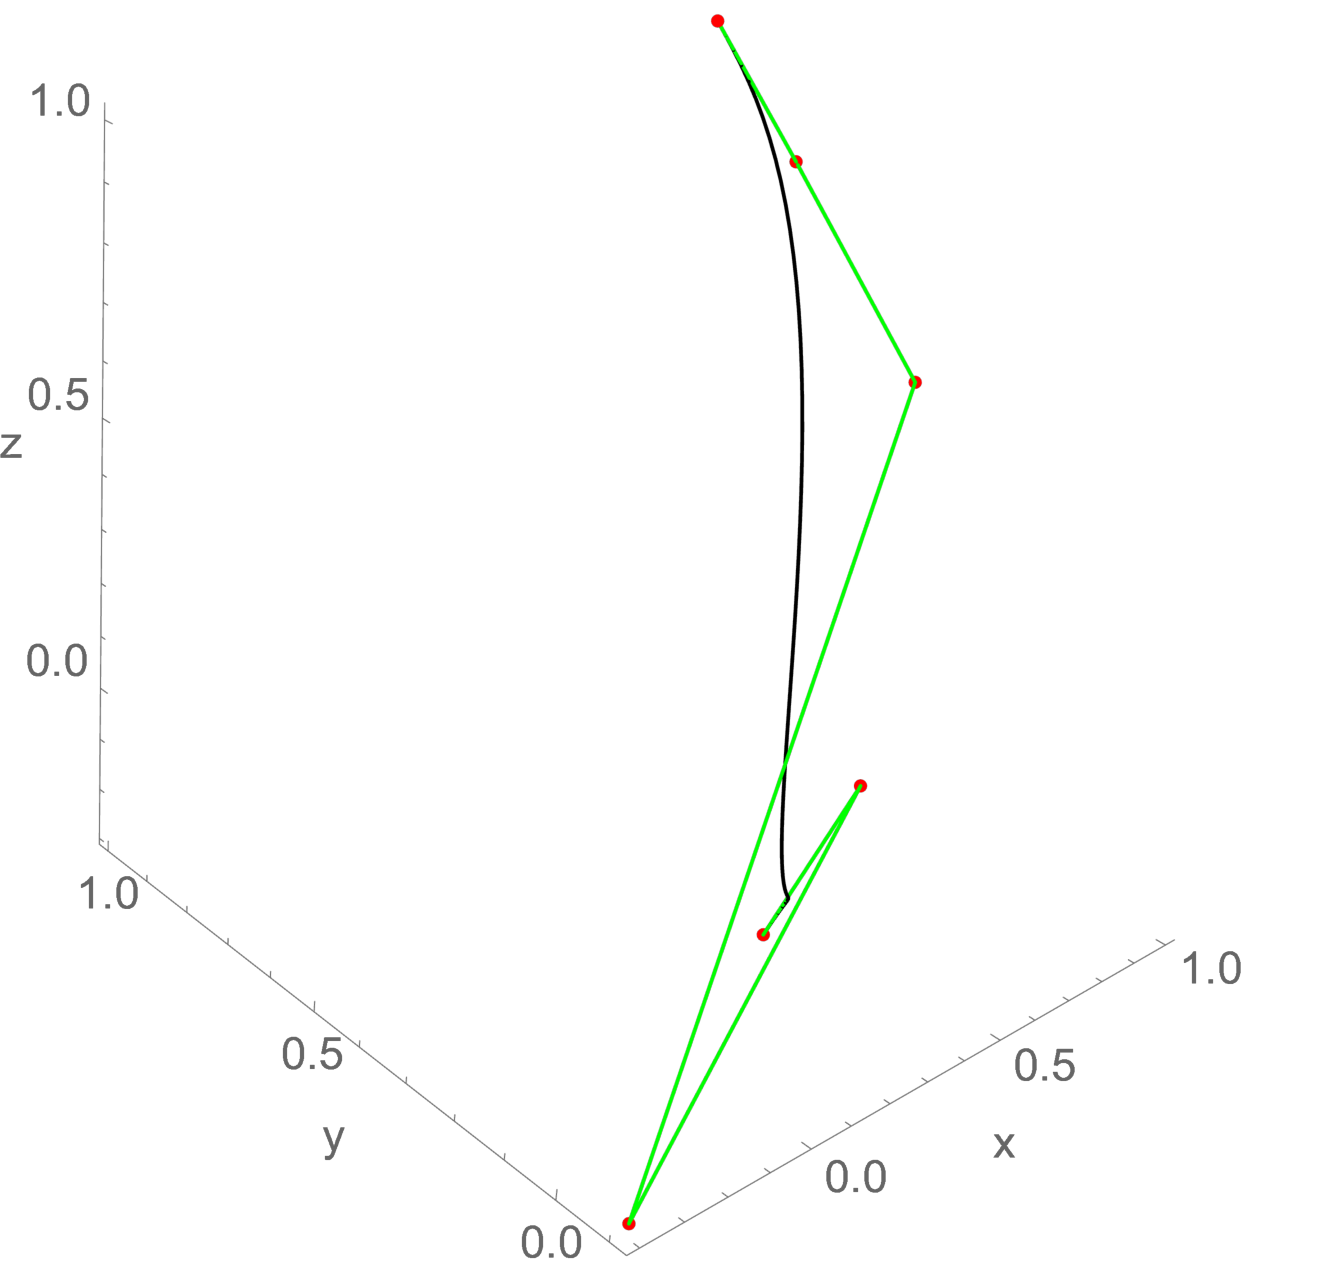
\includegraphics[width=0.3\textwidth]{../latex_datoteke/images/hermit1.pdf}
	  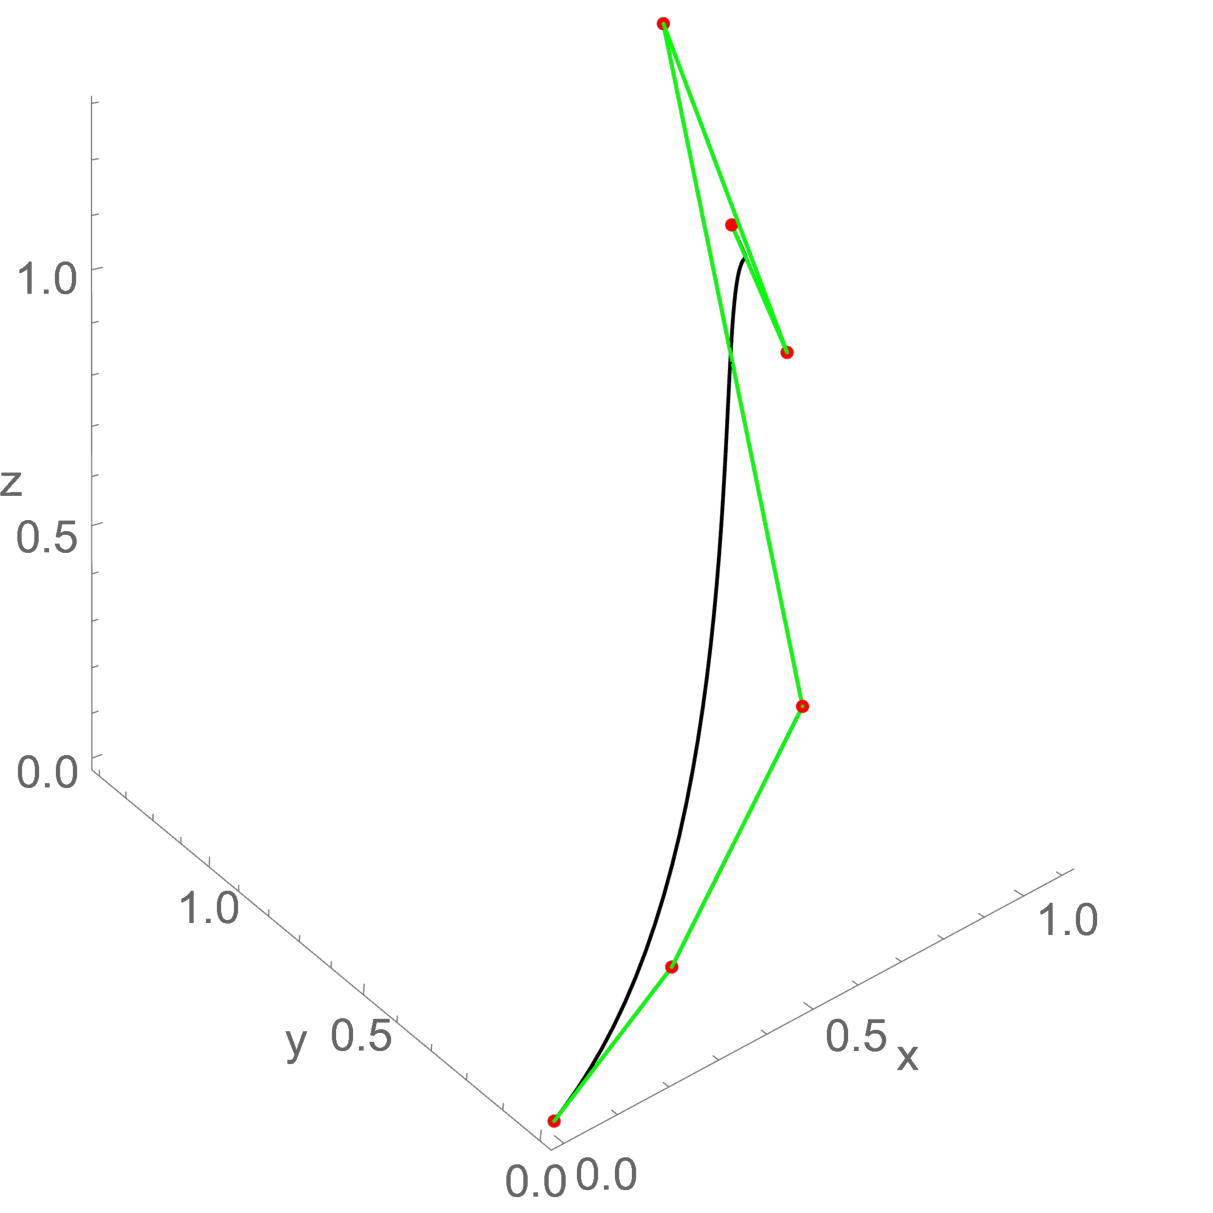
\includegraphics[width=0.3\textwidth]{../latex_datoteke/images/hermit2.pdf}
	  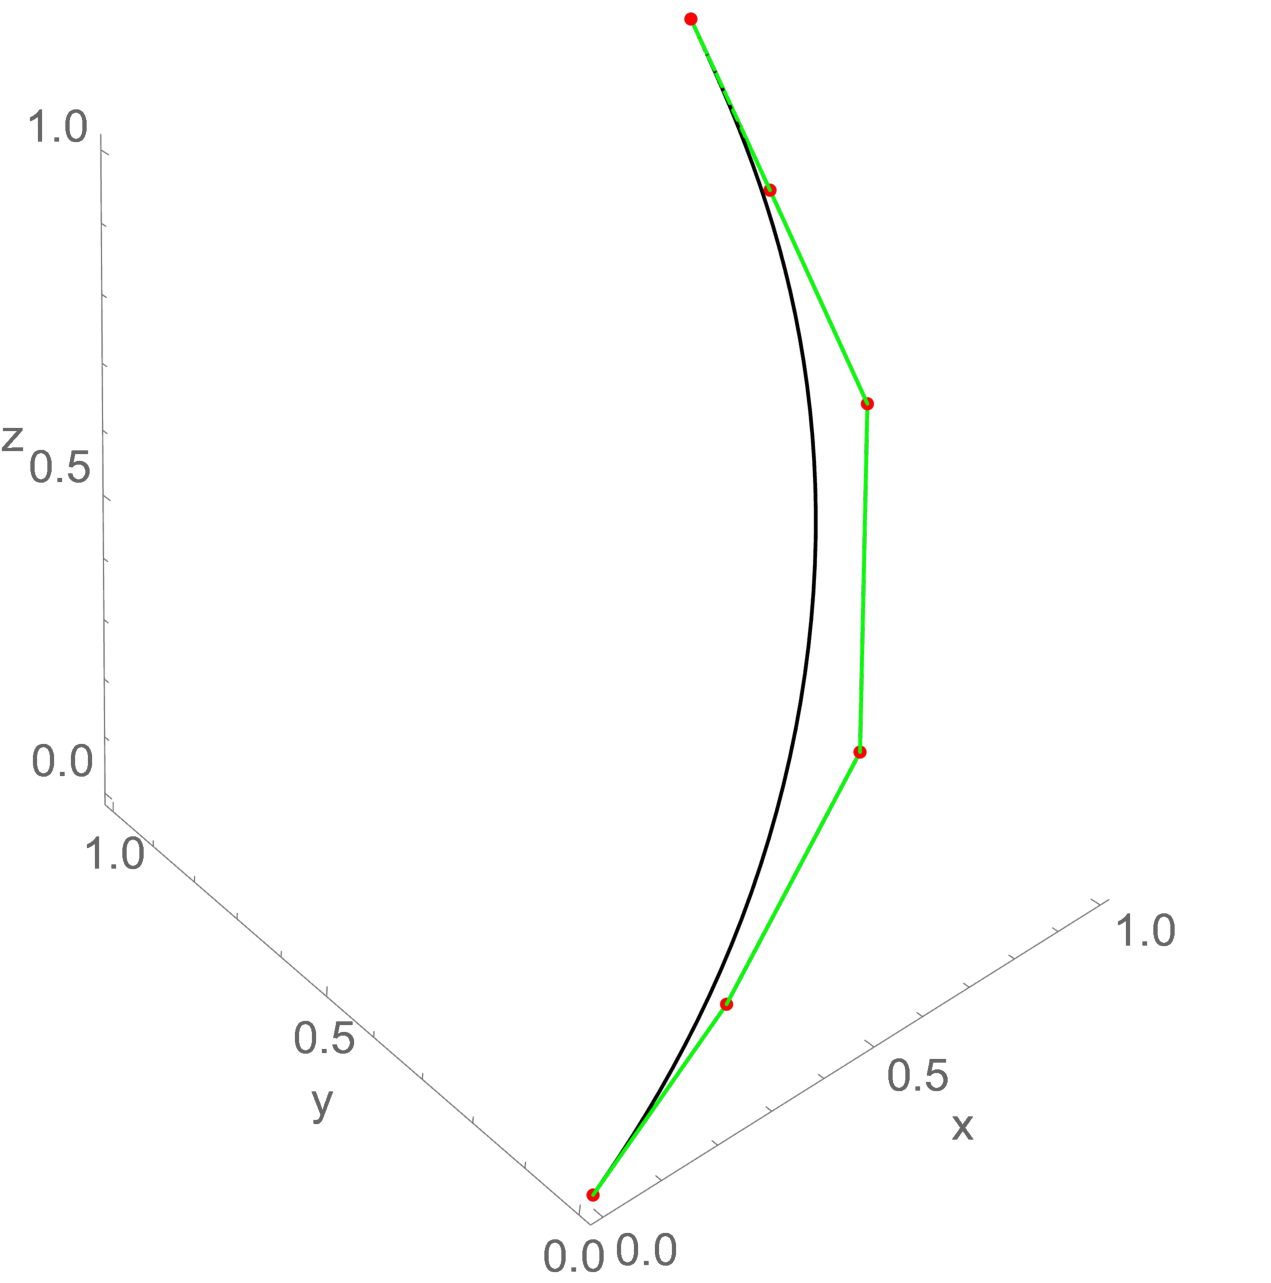
\includegraphics[width=0.3\textwidth]{../latex_datoteke/images/hermit3.pdf}
	  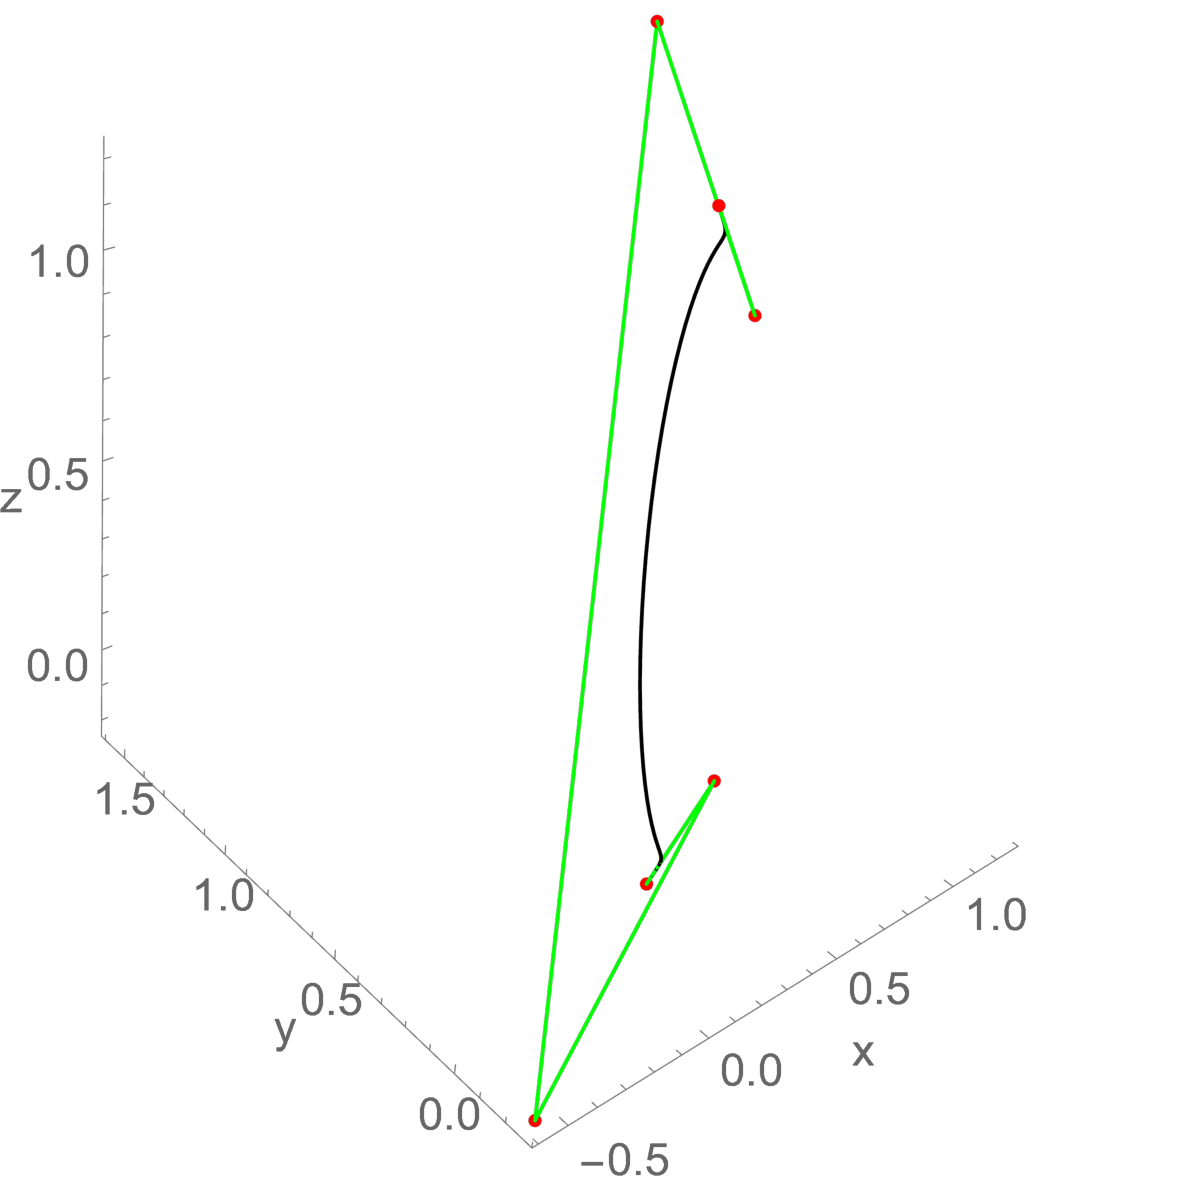
\includegraphics[width=0.3\textwidth]{../latex_datoteke/images/hermit4.pdf}
	% \caption[caption za v kazalo]{Dolg caption pod sliko}
	  \caption[Interpolacijske DPH krivulje]{Štiri interpolacijske DPH krivulje s pripadajočimi kontrolnimi poligoni za podatke $\pV_i=(0,0,0),$ $\pV_f=(1,1,1),$ $\dV_i=(1,0,1)$ in $\dV_f=(0,1,1).$}
	  \label{hermit_grafi_krivulj}
	\end{figure}
}
%%%%%%%%%%%%%%%%%%%%%%%%%%%%%%%%%%%%%%%%%%%%
\end{document}
